\documentclass[12pt,twoside]{article}

\newcommand{\reporttitle}{Markowitz Model \& Rolling Window Back-Testing}
\newcommand{\reportauthor}{Edward Peterson}
\newcommand{\reporttype}{Computational Finance with C++}
\newcommand{\cid}{01502703}

% include files that load packages and define macros
%%%%%%%%%%%%%%%%%%%%%%%%%%%%%%%%%%%%%%%%%
% University Assignment Title Page 
% LaTeX Template
% Version 1.0 (27/12/12)
%
% This template has been downloaded from:
% http://www.LaTeXTemplates.com
%
% Original author:
% WikiBooks (http://en.wikibooks.org/wiki/LaTeX/Title_Creation)
%
% License:
% CC BY-NC-SA 3.0 (http://creativecommons.org/licenses/by-nc-sa/3.0/)
% 
% Instructions for using this template:
% This title page is capable of being compiled as is. This is not useful for 
% including it in another document. To do this, you have two options: 
%
% 1) Copy/paste everything between \begin{document} and \end{document} 
% starting at \begin{titlepage} and paste this into another LaTeX file where you 
% want your title page.
% OR
% 2) Remove everything outside the \begin{titlepage} and \end{titlepage} and 
% move this file to the same directory as the LaTeX file you wish to add it to. 
% Then add \input{./title_page_1.tex} to your LaTeX file where you want your
% title page.
%
%----------------------------------------------------------------------------------------
%   PACKAGES AND OTHER DOCUMENT CONFIGURATIONS
%----------------------------------------------------------------------------------------
\usepackage{ifxetex}
\usepackage{textpos}
\usepackage{natbib}
\usepackage{kpfonts}
\usepackage[a4paper,hmargin=2.8cm,vmargin=2.0cm,includeheadfoot]{geometry}
\usepackage{ifxetex}
\usepackage{stackengine}
\usepackage{tabularx,longtable,multirow,subfigure,caption}%hangcaption
\usepackage{fncylab} %formatting of labels
\usepackage{fancyhdr}
\usepackage{color}
\usepackage[tight,ugly]{units}
\usepackage{url}
\usepackage{float}
\usepackage[english]{babel}
\usepackage{amsmath}
\usepackage{graphicx}
\usepackage[colorinlistoftodos]{todonotes}
\usepackage{dsfont}
\usepackage{epstopdf} % automatically replace .eps with .pdf in graphics
\usepackage{natbib}
\usepackage{backref}
\usepackage{array}
\usepackage{latexsym}
\usepackage{etoolbox}

\usepackage{enumerate} % for numbering with [a)] format 



\ifxetex
\usepackage{fontspec}
\setmainfont[Scale=.8]{OpenDyslexic-Regular}
\else
\usepackage[pdftex,pagebackref,hypertexnames=false,colorlinks]{hyperref} % provide links in pdf
\hypersetup{pdftitle={},
  pdfsubject={}, 
  pdfauthor={\reportauthor},
  pdfkeywords={}, 
  pdfstartview=FitH,
  pdfpagemode={UseOutlines},% None, FullScreen, UseOutlines
  bookmarksnumbered=true, bookmarksopen=true, colorlinks,
    citecolor=black,%
    filecolor=black,%
    linkcolor=black,%
    urlcolor=black}
\usepackage[all]{hypcap}
\fi

\usepackage{tcolorbox}

% various theorems
\usepackage{ntheorem}
\theoremstyle{break}
\newtheorem{lemma}{Lemma}
\newtheorem{theorem}{Theorem}
\newtheorem{remark}{Remark}
\newtheorem{definition}{Definition}
\newtheorem{proof}{Proof}

% example-environment
\newenvironment{example}[1][]
{ 
\vspace{4mm}
\noindent\makebox[\linewidth]{\rule{\hsize}{1.5pt}}
\textbf{Example #1}\\
}
{ 
\noindent\newline\makebox[\linewidth]{\rule{\hsize}{1.0pt}}
}



%\renewcommand{\rmdefault}{pplx} % Palatino
% \renewcommand{\rmdefault}{put} % Utopia

\ifxetex
\else
\renewcommand*{\rmdefault}{bch} % Charter
\renewcommand*{\ttdefault}{cmtt} % Computer Modern Typewriter
%\renewcommand*{\rmdefault}{phv} % Helvetica
%\renewcommand*{\rmdefault}{iwona} % Avant Garde
\fi

\setlength{\parindent}{0em}  % indentation of paragraph

\setlength{\headheight}{14.5pt}
\pagestyle{fancy}
\fancyfoot[ER,OL]{\thepage}%Page no. in the left on
                                %odd pages and on right on even pages
\fancyfoot[OC,EC]{\sffamily }
\renewcommand{\headrulewidth}{0.1pt}
\renewcommand{\footrulewidth}{0.1pt}
\captionsetup{margin=10pt,font=small,labelfont=bf}


%--- chapter heading

\def\@makechapterhead#1{%
  \vspace*{10\p@}%
  {\parindent \z@ \raggedright %\sffamily
        %{\Large \MakeUppercase{\@chapapp} \space \thechapter}
        %\\
        %\hrulefill
        %\par\nobreak
        %\vskip 10\p@
    \interlinepenalty\@M
    \Huge \bfseries 
    \thechapter \space\space #1\par\nobreak
    \vskip 30\p@
  }}

%---chapter heading for \chapter*  
\def\@makeschapterhead#1{%
  \vspace*{10\p@}%
  {\parindent \z@ \raggedright
    \sffamily
    \interlinepenalty\@M
    \Huge \bfseries  
    #1\par\nobreak
    \vskip 30\p@
  }}
  



% %%%%%%%%%%%%% boxit
\def\Beginboxit
   {\par
    \vbox\bgroup
       \hrule
       \hbox\bgroup
          \vrule \kern1.2pt %
          \vbox\bgroup\kern1.2pt
   }

\def\Endboxit{%
                  \kern1.2pt
               \egroup
          \kern1.2pt\vrule
        \egroup
       \hrule
     \egroup
   }    

\newenvironment{boxit}{\Beginboxit}{\Endboxit}
\newenvironment{boxit*}{\Beginboxit\hbox to\hsize{}}{\Endboxit}



\allowdisplaybreaks

\makeatletter
\newcounter{elimination@steps}
\newcolumntype{R}[1]{>{\raggedleft\arraybackslash$}p{#1}<{$}}
\def\elimination@num@rights{}
\def\elimination@num@variables{}
\def\elimination@col@width{}
\newenvironment{elimination}[4][0]
{
    \setcounter{elimination@steps}{0}
    \def\elimination@num@rights{#1}
    \def\elimination@num@variables{#2}
    \def\elimination@col@width{#3}
    \renewcommand{\arraystretch}{#4}
    \start@align\@ne\st@rredtrue\m@ne
}
{
    \endalign
    \ignorespacesafterend
}
\newcommand{\eliminationstep}[2]
{
    \ifnum\value{elimination@steps}>0\leadsto\quad\fi
    \left[
        \ifnum\elimination@num@rights>0
            \begin{array}
            {@{}*{\elimination@num@variables}{R{\elimination@col@width}}
            |@{}*{\elimination@num@rights}{R{\elimination@col@width}}}
        \else
            \begin{array}
            {@{}*{\elimination@num@variables}{R{\elimination@col@width}}}
        \fi
            #1
        \end{array}
    \right]
    & 
    \begin{array}{l}
        #2
    \end{array}
    &%                                    moved second & here
    \addtocounter{elimination@steps}{1}
}
\makeatother

%% Fast macro for column vectors
\makeatletter  
\def\colvec#1{\expandafter\colvec@i#1,,,,,,,,,\@nil}
\def\colvec@i#1,#2,#3,#4,#5,#6,#7,#8,#9\@nil{% 
  \ifx$#2$ \begin{bmatrix}#1\end{bmatrix} \else
    \ifx$#3$ \begin{bmatrix}#1\\#2\end{bmatrix} \else
      \ifx$#4$ \begin{bmatrix}#1\\#2\\#3\end{bmatrix}\else
        \ifx$#5$ \begin{bmatrix}#1\\#2\\#3\\#4\end{bmatrix}\else
          \ifx$#6$ \begin{bmatrix}#1\\#2\\#3\\#4\\#5\end{bmatrix}\else
            \ifx$#7$ \begin{bmatrix}#1\\#2\\#3\\#4\\#5\\#6\end{bmatrix}\else
              \ifx$#8$ \begin{bmatrix}#1\\#2\\#3\\#4\\#5\\#6\\#7\end{bmatrix}\else
                 \PackageError{Column Vector}{The vector you tried to write is too big, use bmatrix instead}{Try using the bmatrix environment}
              \fi
            \fi
          \fi
        \fi
      \fi
    \fi
  \fi 
}  
\makeatother

\robustify{\colvec}

%%% Local Variables: 
%%% mode: latex
%%% TeX-master: "notes"
%%% End: 
 % various packages needed for maths etc.
% quick way of adding a figure
\newcommand{\fig}[3]{
 \begin{center}
  \scalebox{#3}{\includegraphics[#2]{#1}}
   \end{center}
   }

   %\newcommand*{\point}[1]{\vec{\mkern0mu#1}}
   \newcommand{\ci}[0]{\perp\!\!\!\!\!\perp} % conditional independence
   \newcommand{\point}[1]{{#1}} % points 
   \renewcommand{\vec}[1]{{\boldsymbol{{#1}}}} % vector
   \newcommand{\mat}[1]{{\boldsymbol{{#1}}}} % matrix
   \newcommand{\R}[0]{\mathds{R}} % real numbers
   \newcommand{\Z}[0]{\mathds{Z}} % integers
   \newcommand{\N}[0]{\mathds{N}} % natural numbers
   \newcommand{\nat}[0]{\mathds{N}} % natural numbers
   \newcommand{\Q}[0]{\mathds{Q}} % rational numbers
   \ifxetex
   \newcommand{\C}[0]{\mathds{C}} % complex numbers
   \else
   \newcommand{\C}[0]{\mathds{C}} % complex numbers
   \fi
   \newcommand{\tr}[0]{\text{tr}} % trace
   \renewcommand{\d}[0]{\mathrm{d}} % total derivative
   \newcommand{\inv}{^{-1}} % inverse
   \newcommand{\id}{\mathrm{id}} % identity mapping
   \renewcommand{\dim}{\mathrm{dim}} % dimension
   \newcommand{\rank}[0]{\mathrm{rk}} % rank
   \newcommand{\determ}[1]{\mathrm{det}(#1)} % determinant
   \newcommand{\scp}[2]{\langle #1 , #2 \rangle}
   \newcommand{\kernel}[0]{\mathrm{ker}} % kernel/nullspace
   \newcommand{\img}[0]{\mathrm{Im}} % image
   \newcommand{\idx}[1]{{(#1)}}
   \DeclareMathOperator*{\diag}{diag}
   \newcommand{\E}{\mathds{E}} % expectation
   \newcommand{\var}{\mathds{V}} % variance
   \newcommand{\gauss}[2]{\mathcal{N}\big(#1,\,#2\big)} % gaussian distribution N(.,.)
   \newcommand{\gaussx}[3]{\mathcal{N}\big(#1\,|\,#2,\,#3\big)} % gaussian distribution N(.|.,.)
   \newcommand{\gaussBig}[2]{\mathcal{N}\left(#1,\,#2\right)} % see above, but with brackets that adjust to the height of the arguments
   \newcommand{\gaussxBig}[3]{\mathcal{N}\left(#1\,|\,#2,\,#3\right)} % see above, but with brackets that adjust to the height of the arguments
   \DeclareMathOperator{\cov}{Cov} % covariance (matrix) 
   \ifxetex
   \renewcommand{\T}[0]{^\top} % transpose
   \else
   \newcommand{\T}[0]{^\top}
   \fi
   % matrix determinant
   \newcommand{\matdet}[1]{
   \left|
   \begin{matrix}
   #1
   \end{matrix}
   \right|
   }



   %%% various color definitions
   \definecolor{darkgreen}{rgb}{0,0.6,0}

   \newcommand{\blue}[1]{{\color{blue}#1}}
   \newcommand{\red}[1]{{\color{red}#1}}
   \newcommand{\green}[1]{{\color{darkgreen}#1}}
   \newcommand{\orange}[1]{{\color{orange}#1}}
   \newcommand{\magenta}[1]{{\color{magenta}#1}}
   \newcommand{\cyan}[1]{{\color{cyan}#1}}


   % redefine emph
   \renewcommand{\emph}[1]{\blue{\bf{#1}}}

   % place a colored box around a character
   \gdef\colchar#1#2{%
     \tikz[baseline]{%
       \node[anchor=base,inner sep=2pt,outer sep=0pt,fill = #2!20] {#1};
           }%
           }%

 % short-hand notation and macros

\usepackage{hyperref}
\usepackage{enumitem}
\usepackage{tikz}
\usetikzlibrary{arrows.meta, positioning, shapes.geometric}

%%%%%%%%%%%%%%%%%%%%%%%%%%%%

\begin{document}
% front page
% Last modification: 2016-09-29 (Marc Deisenroth)
\begin{titlepage}

\newcommand{\HRule}{\rule{\linewidth}{0.5mm}} % Defines a new command for the horizontal lines, change thickness here


%----------------------------------------------------------------------------------------
%   LOGO SECTION
%----------------------------------------------------------------------------------------


\includegraphics[width = 4cm]{./figures/imperial}\\[0.5cm] 

\begin{center} % Center remainder of the page

%----------------------------------------------------------------------------------------
%   HEADING SECTIONS
%----------------------------------------------------------------------------------------
\textsc{\LARGE \reporttype}\\[1.5cm] 
\textsc{\Large Imperial College London}\\[0.5cm] 
\textsc{\large Department of Computing}\\[0.5cm] 
%----------------------------------------------------------------------------------------
%   TITLE SECTION
%----------------------------------------------------------------------------------------

\HRule \\[0.4cm]
{ \huge \bfseries \reporttitle}\\ % Title of your document
\HRule \\[1.5cm]
\end{center}
%----------------------------------------------------------------------------------------
%   AUTHOR SECTION
%----------------------------------------------------------------------------------------

%\begin{minipage}{0.4\hsize}
\begin{flushleft} \large
\textit{Author:}\\
\reportauthor~(CID: \cid) % Your name
\end{flushleft}
\vspace{2cm}
\makeatletter
Date: \@date 

\vfill % Fill the rest of the page with whitespace



\makeatother


\end{titlepage}




%%%%%%%%%%%%%%%%%%%%%%%%%%%% Main document
\section{Software Structure}
\textbf{\href{https://github.com/ep4518/CFcrsw}{www.github.com/ep4518/CFcrsw}}
\begin{itemize}[nosep]
    \item no use of polymorphism
    \item read\_data.h and read\_data.cpp unchanged
    \item defined type Vector and Lattice as vector$<$double$>$ and vector$<$vector$<$double$>$$>$
    \item defined class ``Matrix" holds a lattice and implements rudimentary linear algebra with multiple constructors available e.g. (rows, columns), (Lattice), ().
    \begin{itemize}[nosep]
        \item operator overload for multiplication, addition, subtraction, unary negative and also for scalar equivalent operations
        \item operator overload for splcing, along with functionallity for insertion, printing, retrieval, shape etc.
        \item ultimately building towards implementing the Conjugate Gradient Descent Solver.
    \end{itemize}
    \item implemented numpy-like horizontal and vertical stacking of Matrix triples
    \item Markowitz class for defining a portfolio with optimal asset weightings
    \begin{itemize}[nosep]
        \item mean() - average returns for each asset over sample period - $\bar{r}_i = \frac{1}{n}\Sigma_{k=1}^n r_{i,k} $
        \item cov() - covariance of asset returns - $\Sigma_{ij} = \frac{1}{n - 1}\sum_{k=1}^n (r_{i,k} - \bar{r}_i)(r_{j,k} - \bar{r}_j)$
        \item b(double target\_return), Q() - vstack(hstack, hstack, hstack)
        \item optimal\_weights(): $Q x = b$
    \end{itemize}
    \item backtesting function called for each iteration in the rolling window
    \item wrote array of result structs in csv form for plotting with python - write\_data.h
\end{itemize}

\vspace{1cm}

% Class Diagram
\begin{tikzpicture}[
    class/.style={rectangle, draw=black, fill=gray!10, rounded corners, 
                  minimum height=2em, minimum width=5em, text centered, 
                  text width=5em},
    class box/.style={rectangle, draw=black, fill=white, rounded corners, 
                      minimum height=2em, minimum width=10em, text centered, 
                      text width=10em, font=\ttfamily},
    relation/.style={-{Stealth}, thin}
]

% Define classes
\node[class] (class1) {Matrix Class};
\node[class, below=of class1, yshift=-1cm] (class2) {Markowitz Class};

% Class contents
\node[class box, right=of class1] (class1Methods) {operator overload \\ - \\ solver() \\ - \\miscLinearAlbegra()};

\node[class box, right=of class2] (class2Methods) {cov() \\ - \\ Q() \\ - \\ OptimalWeights()};



% Relations
\draw[relation] (class1) -- (class2);

\end{tikzpicture}

% Sequence Diagram
\begin{tikzpicture}[
    actor/.style={rectangle, draw=black, fill=gray!10, rounded corners, 
                  minimum height=2em, minimum width=5em, text centered},
    message/.style={->, thin}
]

% Actors and Objects
\node[actor] (user) {Main};
\node[actor, right=of user, xshift=1cm] (system) {i=0, i=12, ..., i $<$ 600};
\node[actor, right=of system] (third) {Portfolio - In Sample};
\node[actor, below=of third] (fourth) {Backtest};
\node[actor, left=of fourth] (fifth) {Daily Returns - Out of Sample};
\node[actor, above=of third] (sixth) {Target Returns};

% Messages
\draw[message] (user) -- node[below] {loop} (system);
\draw[message] (system) -- node[] {} (third);
\draw[message] (third) -- node[] {} (fourth);
\draw[message] (fifth) -- node[] {} (fourth);
\draw[message] (fourth) -- node[] {} (system);
\draw[message] (sixth) -- node[] {} (third);
\draw[message] (user) -- node[] {} (sixth);

\end{tikzpicture}

\section{Evaluation}

\begin{figure}[htbp!]
\centering
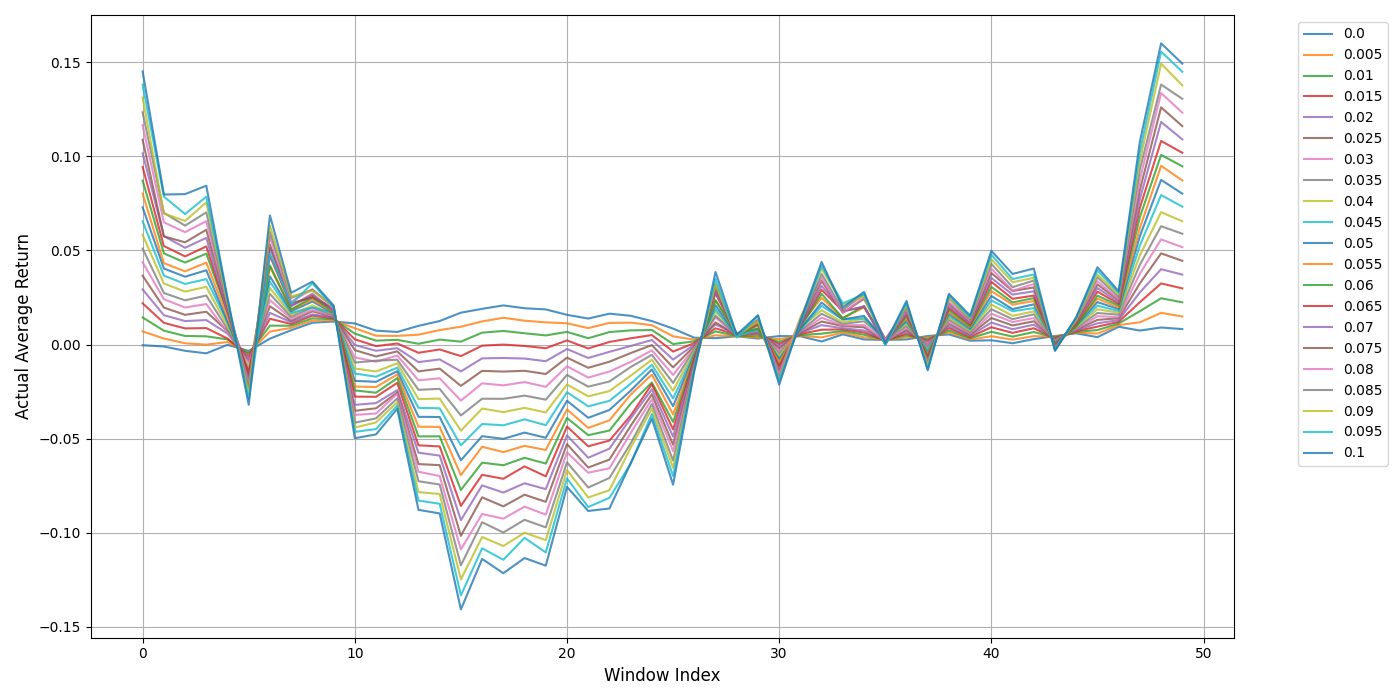
\includegraphics[width = 1.0\hsize]{./figures/Realised_Rolling_Window_Average_OOS_Return_cpp.png} % span 1.0 times the horizontal size of the page
\caption{Realised Rolling Window Average OOS Return for each Target} 
\label{fig:OOS_rets}
\end{figure}


Fig.~\ref{fig:OOS_rets} portrays the rolling window realised average return for each target over the course of the backtest. There are 50 periods in the backtest indexed on the x-axis of the plot. Out of sample performance of the Markowtiz model is poor. The cumulative performance over the enitre domain is slightly better the larger the target return becomes (Fig. ~\ref{fig:cuml_rets}); the overall cumulative performance is positive.\\

\begin{figure}[]
\centering 
\includegraphics[width = 1.0\hsize]{./figures/Cumulative_returns.png} 
\caption{Cumulative 12-day Out of Sample Returns of Optimal Portfolios (No Frictions)}
\label{fig:cuml_rets}
\end{figure}

To evaluate the accuracy of our Markowitz implementation (Fig.~\ref{fig:OOS_rets}), we contrast with a numpy analog, where the linalg library provides a relaible solver to compare the accuracy of the conjugate gradient descent algorithm (CGD) in cpp. Fig.~\ref{fig:OOS_rets_python} shows the drastic impact of the fractional differences in optimal weights we see whilst solving with CGD, on the overall performance during the backtesting phase. Following extensive debugging, these differences were also observed in the Matlab conjgrad.m implementation. Any CGD solver used had $\lVert Qx - b \rVert \thickapprox e^{-5}$ for the range of target returns during backtesting (Fig.~\ref{fig:Matlab}), where as for prebuilt solvers the norm value usually lies in the range $\thickapprox e^{-11}$. \\

In both cases, the Markowitz portfolio effectively captures the market Beta, and produces returns that scale consistently with the amount of risk taken by the investor (Fig.~\ref{fig:eff_front_all}); where the magnitude and direction of those returns is dictated by those of the market. Fig.~\ref{fig:efficint_frontier} demonstrates the Sharpe ratio of the portfolios for an example backtest period. In general, we observed this classic efficient frontier shape in most periods, allowing for inversion in periods of negative market returns. 
\\

Fig.~\ref{fig:Cumulative_Rets} portrays a cumulative portfolio return next to its constituent assets. As with Fig.~\ref{fig:efficint_frontier}, this figure is an example and has been selected with bias.

\begin{figure}[]
    \centering
    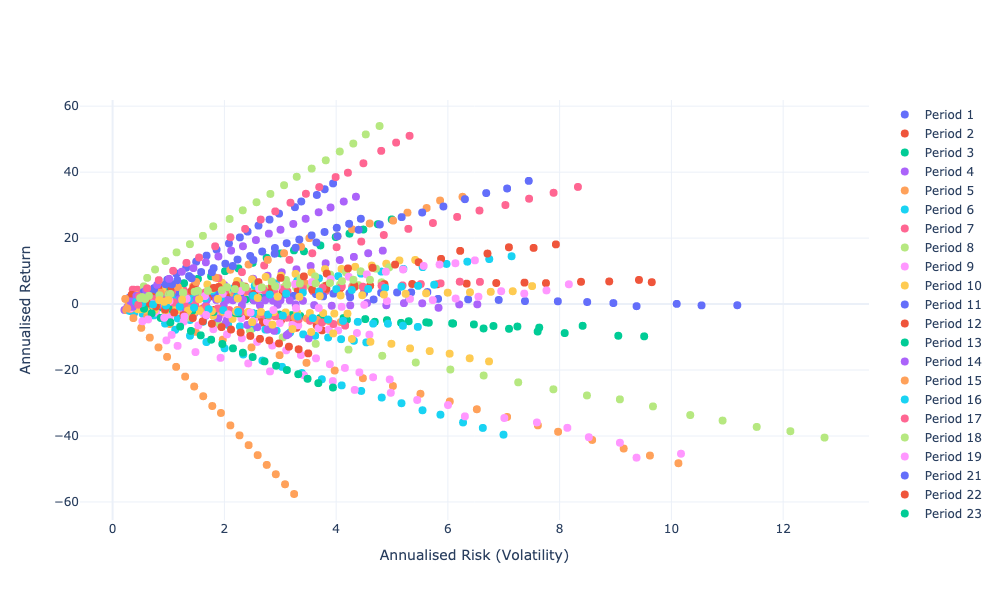
\includegraphics[width = 1.0\hsize]{./figures/efficient_frontier_all_periods.png}
    \caption{Efficient Frontier with Optimal Portfolios (All Backtest Periods [1,50])}
    \label{fig:eff_front_all}
\end{figure}

\newpage
\section{Appendix}
\begin{figure}[htbp!]
    \centering 
    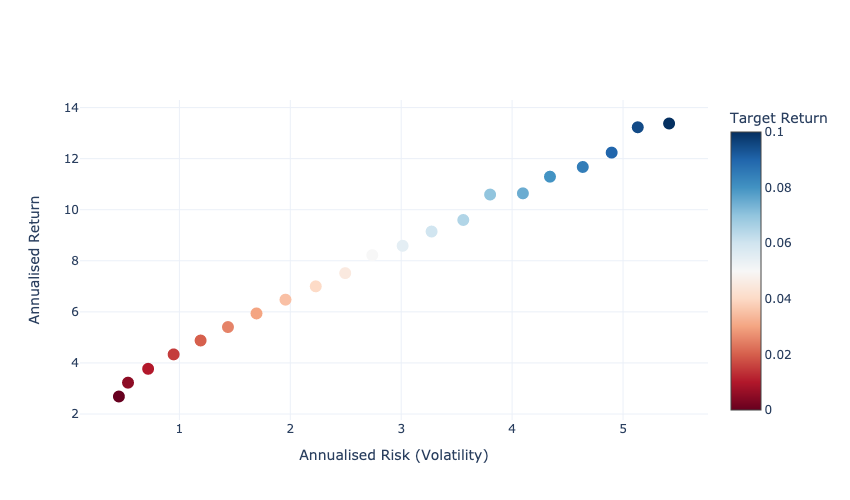
\includegraphics[width = 1.0\hsize]{./figures/efficint_frontier.png} 
    \caption{Efficient Frontier with Optimal Portfolios (Backtest Period 9)} 
\label{fig:efficint_frontier}
\end{figure}
\begin{figure}[htbp!]
    \centering
    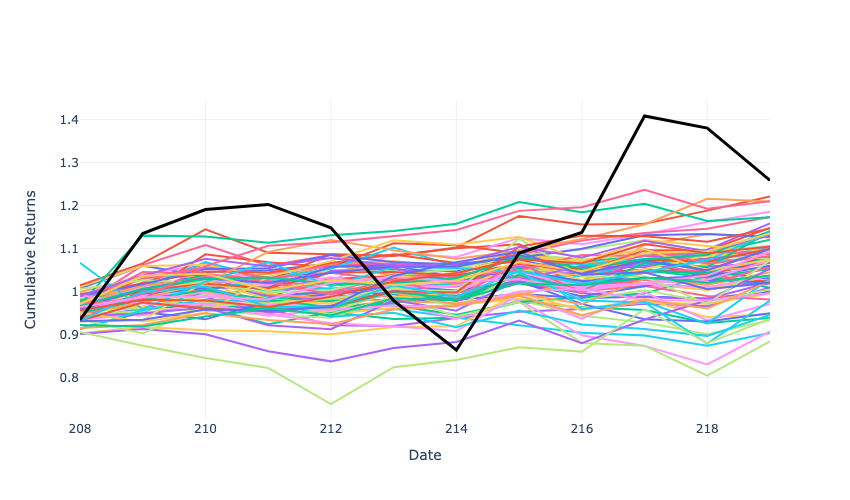
\includegraphics[width = 1.0\hsize]{./figures/Cumulative_Rets.png}
    \caption{Cumulative Returns of Optimized Portfolio vs. Assets (Backtest Period 9, Target R 0.04)}
\label{fig:Cumulative_Rets}
\end{figure}
\begin{figure}[htbp!]
\centering
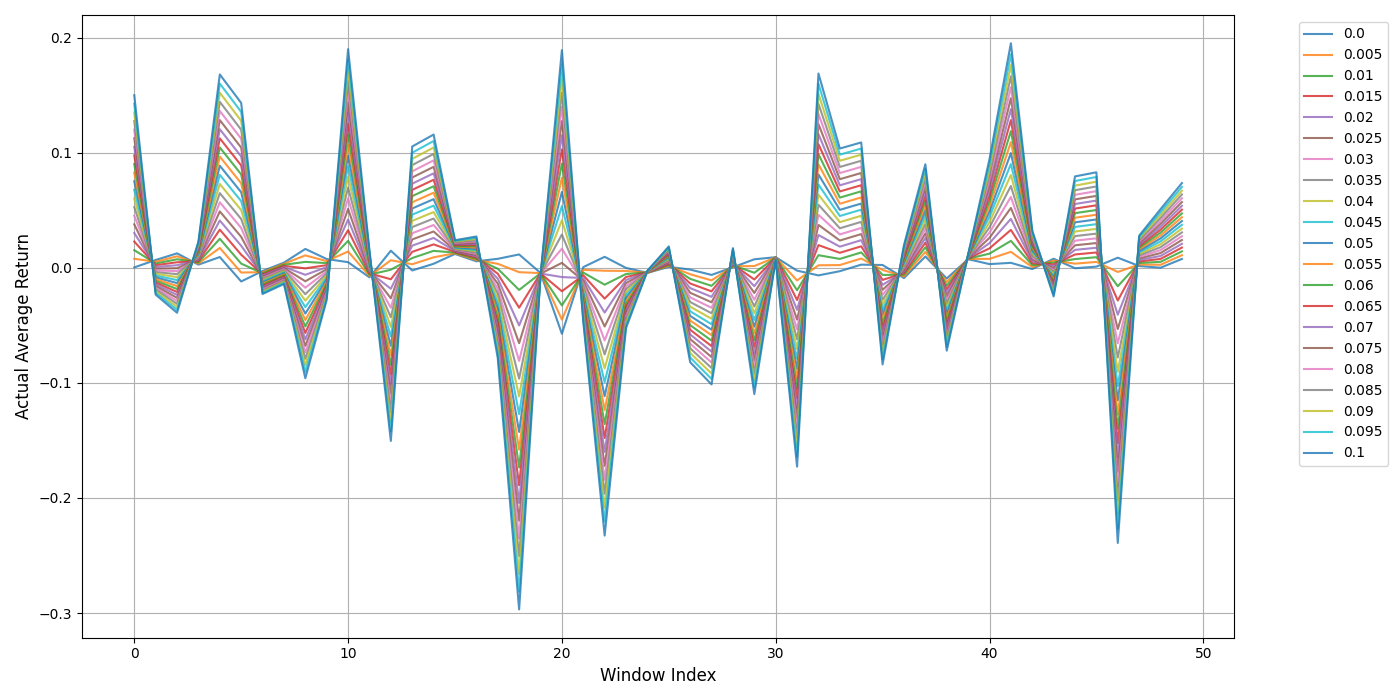
\includegraphics[width = 1.0\hsize]{./figures/Realised_Rolling_Window_Average_OOS_Return.png} 
\caption{Realised Rolling Window Average OOS Return for each Target - Python} 
\label{fig:OOS_rets_python}
\end{figure}
\begin{figure}[htbp!]
    \centering
    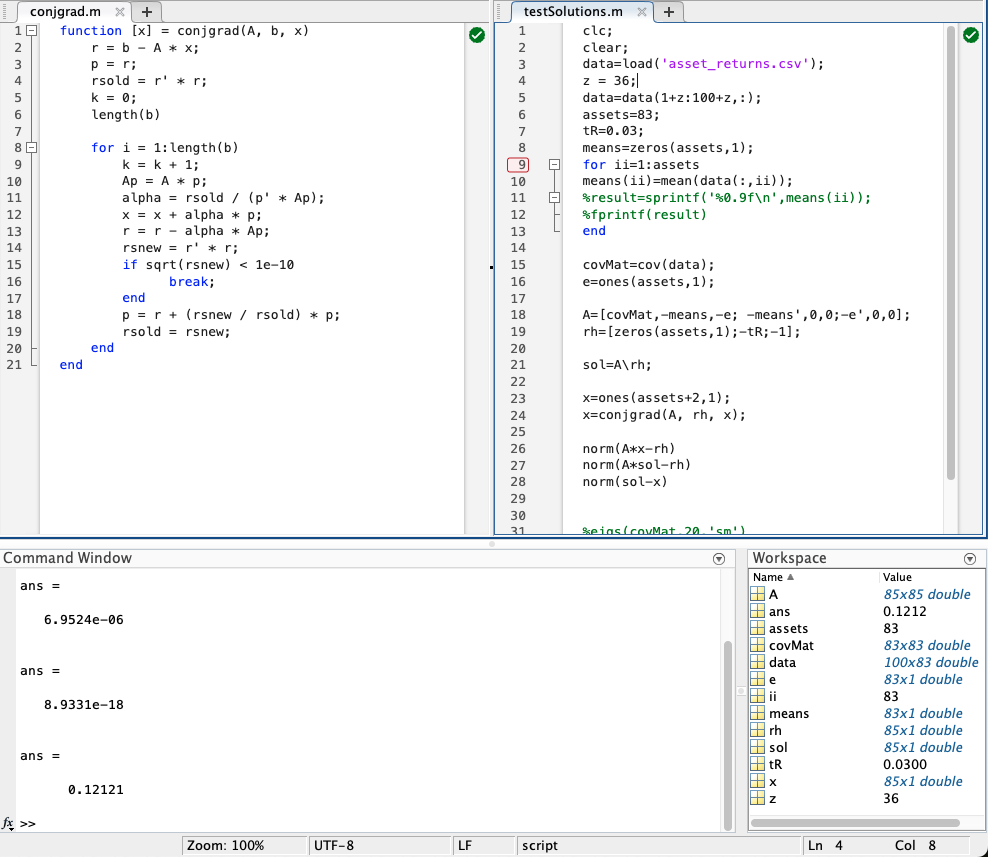
\includegraphics[width = 1.0\hsize]{./figures/ss.png}
    \caption{Matlab}
\label{fig:Matlab}
\end{figure}

\newpage
\subsection{Code}
\textbf{\href{https://github.com/ep4518/CFcrsw}{www.github.com/ep4518/CFcrsw}}
\begin{itemize}
    \item main.cpp
    \item csv.cpp
    \item read\_data.cpp
    \item linalg.cpp
    \item Markowitz.cpp
    \item write\_data.cpp
\end{itemize}
\subsubsection{main.cpp}
\scriptsize
\begin{verbatim}
// main.cpp
#include "read_data.h"
#include "write_data.h"
#include "linalg.h"
#include "Markowitz.h"
#include <iostream>

using namespace std;

// A function to implement a backtest for each window. Takes as input the optimal weights from the IS returns,
// the Out of Sample returns, and the target_returns which is linspace(0,21,0.1)
Matrix back_testing(const Matrix &optimal_weights, const Matrix &OOS_returns, const Matrix &target_returns);

// command line arguments unused. Please use cmake to compile and run.
int  main (int  argc, char  *argv[])
{

    int numberAssets=83;
    int numberReturns=700;

    // Lattice is defined in linalg.h, as is Vector
    Lattice returnMatrix(numberAssets, Vector(numberReturns)); // a matrix to store the return data

    //read the data from the file and store it into the return matrix
    string fileName="asset_returns.csv";
    readData(returnMatrix,fileName);          // returnMatrix[i][j] stores the asset i, return j value

    Matrix daily_returns(returnMatrix); // (Assets -> r) * (Days -> c) == 83 * 700

    // np.linspace(0,21,0.1) ==
    Lattice tr =  {
            {0.   , 0.005, 0.01 , 0.015, 0.02 , 0.025, 0.03 , 0.035, 0.04 ,
            0.045, 0.05 , 0.055, 0.06 , 0.065, 0.07 , 0.075, 0.08 , 0.085,
            0.09 , 0.095, 0.1}
    };

    // Matrix object constructed with Lattice => see linalg.h
    Matrix target_returns(tr);

    Matrix daily_returns_test = daily_returns(0, numberAssets, 360, 460);
    Markowitz portfolio(daily_returns_test, target_returns);
    portfolio.NormTest();

    // results array of size number of windows of Result structs.
    // Result struct defined in write_data.h
    Result results[50];
    for (int i = 0; i < numberReturns - 100; i += 12) {             
    // iterating over the starts of each in sample window
        int index = int(i/12);
        // for the results array
        cout << "Moving to index " << index << endl;
        int start = index, mid = index + 100, end = index + 112; // start of IS, start of OOS, end of OOS
        Matrix daily_returns_IS = daily_returns(0, numberAssets, start, mid); // splice => see linalg.h
        Matrix daily_returns_OOS = daily_returns(0, numberAssets, mid, end);
        Markowitz portfolio(daily_returns_IS, target_returns);     // Markowitz class => see Markowitz.h
        Matrix df_optimal_weights = portfolio.getWeights();            
        // calculate optimal porfolio weights using CGD method of Matrix object
        // df_act_returns is 21 * 3 Matrix object that contains target return,
        // actual return and portfolio covariance for each target return
        Matrix df_act_returns = back_testing(df_optimal_weights, daily_returns_OOS, target_returns);
        results[index] = {
                index,
                df_act_returns,
                df_optimal_weights
        };
    }

    results[0].back_test.prn();

    write_data(results, 50);

    return 0;
}

Matrix back_testing(const Matrix &optimal_weights, const Matrix &OOS_returns, const Matrix &target_returns) {
    int num_targ_rets = optimal_weights.getRows();
    int num_assets = OOS_returns.getRows();
    Markowitz OOS_rets(OOS_returns, target_returns);
    // Result matrix to store performance for each set of weights
    Matrix results(num_targ_rets, 3);

    for (int i = 0; i < num_targ_rets; i++) {
        // Extracts the i-th row of optimal weights
        Matrix optimal_weights_row(num_assets, 1);
        for (int j = 0; j < num_assets; j++) {
            optimal_weights_row.insert(j, 0, optimal_weights(i, j));
        }
        Matrix act_ave_return = OOS_rets.mean().transpose() * optimal_weights_row;
        Matrix pf_cov = optimal_weights_row.transpose() * OOS_rets.cov() * optimal_weights_row;
        results.insert(i, 0, target_returns(0,i));
        results.insert(i, 1, act_ave_return(0,0));
        results.insert(i, 2, pf_cov(0,0));
    }
    return results;
}
\end{verbatim}
\subsubsection{csv.cpp}
\scriptsize
\begin{verbatim}
//csv.h
#ifndef _CSV_H
#define _CSV_H

#include <iostream>
#include <algorithm>
#include <string>
#include <vector>

using namespace std;

class Csv {	// read and parse comma-separated values
	// sample input: "LU",86.25,"11/4/1998","2:19PM",+4.0625
	
public:
	Csv(istream& fin = cin, string sep = ",") : 
	fin(fin), fieldsep(sep) {}
	
	int getline(string&);
	string getfield(int n);
	int getnfield() const { return nfield; }
	
private:
	istream& fin;			// input file pointer
	string line;			// input line
	vector<string> field;	// field strings
	int nfield;				// number of fields
	string fieldsep;		// separator characters
	
	int split();
	int endofline(char);
	int advplain(const string& line, string& fld, int);
	int advquoted(const string& line, string& fld, int);
};

#endif

//csv.cpp
#include "csv.h"

// endofline: check for and consume \r, \n, \r\n, or EOF
int Csv::endofline(char c)
{
	int eol;
	
	eol = (c=='\r' || c=='\n');
	if (c == '\r') {
		fin.get(c);
		if (!fin.eof() && c != '\n')
			fin.putback(c);	// read too far
	}
	return eol;
}

// getline: get one line, grow as needed
int Csv::getline(string& str)
{	
	char c;
	
	for (line = ""; fin.get(c) && !endofline(c); )
		line += c;
	split();
	str = line;
	return !fin.eof();
}

// split: split line into fields
int Csv::split()
{
	string fld;
	int i, j;
	
	nfield = 0;
	if (line.length() == 0)
		return 0;
	i = 0;
	
	do {
		if (i < line.length() && line[i] == '"')
			j = advquoted(line, fld, ++i);	// skip quote
		else
			j = advplain(line, fld, i);
		if (nfield >= field.size())
			field.push_back(fld);
		else
			field[nfield] = fld;
		nfield++;
		i = j + 1;
	} while (j < line.length());
	
	return nfield;
}

// advquoted: quoted field; return index of next separator
int Csv::advquoted(const string& s, string& fld, int i)
{
	int j;
	
	fld = "";
	for (j = i; j < s.length(); j++) {
		if (s[j] == '"' && s[++j] != '"') {
			int k = s.find_first_of(fieldsep, j);
			if (k > s.length())	// no separator found
				k = s.length();
			for (k -= j; k-- > 0; )
				fld += s[j++];
			break;
		}
		fld += s[j];
	}
	return j;
}

// advplain: unquoted field; return index of next separator
int Csv::advplain(const string& s, string& fld, int i)
{
	int j;
	
	j = s.find_first_of(fieldsep, i); // look for separator
	if (j > s.length())               // none found
		j = s.length();
	fld = string(s, i, j-i);
	return j;
}


// getfield: return n-th field
string Csv::getfield(int n)
{
	if (n < 0 || n >= nfield)
		return "";
	else
		return field[n];
}
\end{verbatim}
\subsubsection{read\_data.cpp}
\scriptsize
\begin{verbatim}
//read_data.h
#ifndef _READ_DATA_H
#define _READ_DATA_H
#include <sstream>
#include <vector>

double string_to_double( const std::string& s );
void readData(std::vector<std::vector<double> >& returnMatrix,std::string fileName);

#endif

//read_data.cpp
#include <fstream>
#include <stdlib.h>
#include <sstream>
#include <vector>
#include "csv.h"

//g++ -c read_data.cpp
// g++ -c csv.cpp
// g++ -o portfolioSolver csv.o read_data.o
// ./portfolioSolver

double string_to_double( const std::string& s )
{
	std::istringstream i(s);
	double x;
	if (!(i >> x))
		return 0;
	return x;
} 

void readData(std::vector<std::vector<double> >& data, string fileName)
{
	char tmp[20];
	ifstream file (strcpy(tmp, fileName.c_str()));
	Csv csv(file);
	string line;
	if (file.is_open())
	{
		int i=0;
		while (csv.getline(line) != 0) {
         	for (int j = 0; j < csv.getnfield(); j++)
            {
               double temp=string_to_double(csv.getfield(j));
               //cout << "Asset " << j << ", Return "<<i<<"="<< temp<<"\n";
               data[j][i]=temp;
            }
            i++;
		}
		
		file.close();
	}
	else {cout <<fileName <<" missing\n";exit(0);}
}
\end{verbatim}
\subsubsection{linalg.cpp}
\scriptsize
\begin{verbatim}
// linalg.h
#ifndef _LINALG_H
#define _LINALG_H

#include <vector>
#include <iostream>

typedef std::vector<double> Vector;
typedef std::vector<Vector> Lattice;

class Matrix {
private:
    int rows, columns;
    Lattice M;
public:
    // Default constructor
    Matrix() : rows(0), columns(0), M() {}

    // Construct from pre-existing Lattice
    Matrix(Lattice _M) {M = _M; rows = _M.size(); columns = _M[0].size();}

    // Construct a zero matrix with given dimensions
    Matrix(int _rows, int _columns) : rows(_rows), columns(_columns), M(_rows, Vector(_columns, 0.0)) {}

    // Access element (const version)
    const double& operator()(size_t i, size_t j) const { return M[i][j]; }

    // Method to insert an element into the matrix
    void insert(size_t i, size_t j, double value) {
        if (i >= rows || j >= columns) {
            throw std::out_of_range("Matrix indices out of range");
        }
        M[i][j] = value;
    }

    // pandas like shape method
    void shape() {printf("(%d, %d)\n",rows, columns);}

    // Get number of rows
    int getRows() const { return rows; }

    // Get number of columns
    int getColumns() const { return columns; }

    // Get the underlying matrix
    const Lattice& getMatrix() const { return M; }

    // Access element (non-const version)
    double& operator()(size_t i, size_t j) {
        if (i >= rows || j >= columns) throw std::out_of_range("Matrix indices out of range");
        return M[i][j];
    }

    // Unary minus operator for matrix
    Matrix operator-() const;

    // Splicing operator
    Matrix operator()(int row_start, int row_end, int col_start, int col_end) const;

    Matrix transpose() const;

    // Skip inversion. Utilise conjugate gradient algorithm (see .pdf/ wiki)
    // Mx = b => x*
    //  https://en.wikipedia.org/wiki/Conjugate_gradient_method
    Matrix solver(const Matrix &b, const double tol, const int debug) const;

    // Matrix multiplication
    friend Matrix operator*(const Matrix& A, const Matrix& B);
    // Scalar multiplication
    friend Matrix operator*(const double& a, const Matrix&A);

    // Matrix addition/ subtraction
    friend Matrix operator+(const Matrix& A, const Matrix& B);
    friend Matrix operator-(const Matrix& A, const Matrix& B);

    // Dot product of two column matrices
    double dot(const Matrix& A) const;

    // Print the matrix
    void prn() const;

    double norm();

};

// hstack and vstack for constructing Q
Matrix vstack(const Matrix &A, const Matrix &B, const Matrix &C);
Matrix hstack(const Matrix &A, const Matrix &B, const Matrix &C);

#endif

//linalg.cpp
#include "linalg.h"
#include <cmath>
#include <stdexcept>
#include <iostream>

void Matrix::prn() const {
    std::cout << "[\n";
    for (const Vector& row : M) {
        std::cout << " [ ";
        for (const double& elem : row) {
            std::cout << elem << " ";
        }
        std::cout << "]\n";
    }
    std::cout << "]\n";
}

Matrix Matrix::operator()(int row_start, int row_end, int col_start, int col_end) const {
    if (row_start < 0 || row_end > rows || col_start < 0 || col_end > columns) {
        throw std::out_of_range("Index out of bounds");
    }
    Lattice result;
    for (int i = row_start; i < row_end; ++i) {
        Vector row;
        for (int j = col_start; j < col_end; ++j) {
            row.push_back(M[i][j]);
        }
        result.push_back(row);
    }
    return Matrix(result);
}

// Transpose of the matrix
Matrix Matrix::transpose() const {
    Lattice transposed(columns, Vector(rows));
    for (size_t i = 0; i < rows; ++i) {
        for (size_t j = 0; j < columns; ++j) {
            transposed[j][i] = M[i][j];
        }
    }
    return {transposed};
}

// Conjugate Gradient Solver
Matrix Matrix::solver(const Matrix &b, const double tol, const int debug) const {
    if (M.empty() || rows != columns) {
        throw std::invalid_argument("Matrix dimensions are not compatible for inversion");
    }
    if (b.getColumns() != 1 || b.getRows() != rows) {
        throw std::invalid_argument("b must be a column vector with the same number of rows as the matrix.");
    }
    Matrix x(Lattice(rows, Vector(1, 1.0)));
    Matrix r = b - (*this) * x;
    Matrix p = r;
    double rsold = r.dot(r);
    double rsnew;
    if (debug == 1) {
        std::cout << "x.norm() " << x.norm() << std::endl;
        std::cout << "r.norm() " << r.norm() << std::endl;
        for (int k = 0; k < b.getRows(); ++k) {
            Matrix Ap = (*this) * p;
            std::cout << "Ap.norm() " << Ap.norm() << std::endl;
            double alpha = rsold / p.dot(Ap);
            std::cout << "alpha " << alpha << std::endl;
            x = x + alpha * p;
            std::cout << "x.norm() " << x.norm() << std::endl;
            r = r - alpha * Ap;
            std::cout << "r.norm() " << r.norm() << std::endl;
            rsnew = r.dot(r);
            std::cout << "rsnew " << rsnew << std::endl;
            if (std::sqrt(rsnew) < tol) break;
            p = r + (rsnew / rsold) * p;
            std::cout << "p.norm() " << p.norm() << std::endl;
            rsold = rsnew;
            std::cout << "rsold " << rsold << std::endl;
        }
    }
    else {
        for (int k = 0; k < b.getRows(); ++k) {
            Matrix Ap = (*this) * p;
            double alpha = rsold / p.dot(Ap);
            x = x + alpha * p;
            r = r - alpha * Ap;
            rsnew = r.dot(r);
            if (std::sqrt(rsnew) < tol) break;
            p = r + (rsnew / rsold) * p;
            rsold = rsnew;
        }
    }

    return x;
}

// Matrix multiplication
Matrix operator*(const Matrix& A, const Matrix& B) {
    if (A.getColumns() != B.getRows()) {
        throw std::invalid_argument("Matrix dimensions must agree for multiplication.");
    }
    Matrix result(A.getRows(), B.getColumns());
    for (int i = 0; i < A.getRows(); ++i) {
        for (int j = 0; j < B.getColumns(); ++j) {
            for (int k = 0; k < A.getColumns(); ++k) {
                result(i, j) += A(i, k) * B(k, j);
            }
        }
    }
    return result;
}

// Matrix addition
Matrix operator+(const Matrix& A, const Matrix& B) {
    if (A.getRows() != B.getRows() || A.getColumns() != B.getColumns()) {
        throw std::invalid_argument("Matrix dimensions must agree for addition.");
    }
    Matrix result(A.getRows(), A.getColumns());
    for (int i = 0; i < A.getRows(); ++i) {
        for (int j = 0; j < A.getColumns(); ++j) {
            result(i, j) = A(i, j) + B(i, j);
        }
    }
    return result;
}

// Matrix subtraction
Matrix operator-(const Matrix& A, const Matrix& B) {
    if (A.getRows() != B.getRows() || A.getColumns() != B.getColumns()) {
        throw std::invalid_argument("Matrix dimensions must agree for subtraction.");
    }
    Matrix result(A.getRows(), A.getColumns());
    for (int i = 0; i < A.getRows(); ++i) {
        for (int j = 0; j < A.getColumns(); ++j) {
            result(i, j) = A(i, j) - B(i, j);
        }
    }
    return result;
}

// Unary - operator for matrix
Matrix Matrix::operator-() const {
    Matrix result(rows, columns);
    for (int i = 0; i < rows; ++i) {
        for (int j = 0; j < columns; ++j) {
            result(i, j) = -M[i][j];
        }
    }
    return result;
}

// Scalar multiplication
Matrix operator*(const double& a, const Matrix& A) {
    Matrix result(A.getRows(), A.getColumns());
    for (int i = 0; i < A.getRows(); ++i) {
        for (int j = 0; j < A.getColumns(); ++j) {
            result(i, j) = a * A(i, j);
        }
    }
    return result;
}

// Dot product of two column matrices
double Matrix::dot(const Matrix& A) const {
    if (columns != 1 || A.getColumns() != 1 || rows != A.getRows()) {
        throw std::invalid_argument("Dot product requires column matrices of the same size.");
    }
    double result = 0.0;
    for (int i = 0; i < rows; ++i) {
        result += M[i][0] * A(i, 0);
    }
    return result;
}

double Matrix::norm() {
    double result = 0.0;
    for (int i = 0; i < rows; i++) {
        result += pow(M[i][0], 2.0);
    }
    return sqrt(result);
}

// Vertical stack of three matrices
Matrix vstack(const Matrix &A, const Matrix &B, const Matrix &C) {
    if (A.getColumns() != B.getColumns() || A.getColumns() != C.getColumns()) {
        throw std::invalid_argument("vstack requires matrices of the same width.");
    }
    int h = A.getRows() + B.getRows() + C.getRows();
    Matrix result(h, A.getColumns());

    for (int i = 0; i < A.getRows(); ++i) {
        for (int j = 0; j < A.getColumns(); ++j) {
            result(i, j) = A(i, j);
        }
    }
    for (int i = 0; i < B.getRows(); ++i) {
        for (int j = 0; j < B.getColumns(); ++j) {
            result(i + A.getRows(), j) = B(i, j);
        }
    }
    for (int i = 0; i < C.getRows(); ++i) {
        for (int j = 0; j < C.getColumns(); ++j) {
            result(i + A.getRows() + B.getRows(), j) = C(i, j);
        }
    }
    return result;
}

// Horizontal stack of three matrices
Matrix hstack(const Matrix &A, const Matrix &B, const Matrix &C) {
    if (A.getRows() != B.getRows() || A.getRows() != C.getRows()) {
        throw std::invalid_argument("hstack requires matrices of the same height.");
    }
    int w = A.getColumns() + B.getColumns() + C.getColumns();
    Matrix result(A.getRows(), w);

    for (int i = 0; i < A.getRows(); ++i) {
        for (int j = 0; j < A.getColumns(); ++j) {
            result(i, j) = A(i, j);
        }
    }
    for (int i = 0; i < B.getRows(); ++i) {
        for (int j = 0; j < B.getColumns(); ++j) {
            result(i, j + A.getColumns()) = B(i, j);
        }
    }
    for (int i = 0; i < C.getRows(); ++i) {
        for (int j = 0; j < C.getColumns(); ++j) {
            result(i, j + A.getColumns() + B.getColumns()) = C(i, j);
        }
    }
    return result;
}
\end{verbatim}
\subsubsection{Markowitz.cpp}
\scriptsize
\begin{verbatim}
//Markowitz.h
#ifndef MARKOWITZ_H
#define MARKOWITZ_H

#include "linalg.h"

#define TOLERANCE 1e-10
typedef enum {NODEBUG, DEBUG};

class Markowitz {
private:
    Matrix returns;
    Matrix target_returns;
    Matrix optimal_weights;
    int n;

public:
    Markowitz(const Matrix &_returns, const Matrix &_target_returns) {
        if (_target_returns.getRows() != 1) {
            throw std::invalid_argument("target returns should be a column vector");
        }
        returns = _returns; target_returns = _target_returns, n = _returns.getRows();
        this->weights();
    }

    // Mean returns
    Matrix mean();

    // Covariance matrix
    Matrix cov();

    // Q matrix
    Matrix Q();

    // b Vector
    Matrix b(const double &target_return);

    // weights dataframe
    Matrix weights();

    Matrix getWeights() {return this->optimal_weights;}

    void NormTest();

};

#endif

//Markowitz.cpp
#include "Markowitz.h"
#include <iostream>

// implement summation in the pdf
Matrix Markowitz::mean() {
    int assets = returns.getRows();
    int days = returns.getColumns();
    Matrix result(assets, 1);
    double mean;
    for (int i = 0; i < assets; i++) {
        mean = 0;
        for (int j = 0; j < days; j++)
            mean += returns(i, j);
        mean /= days;
        result.insert(i, 0, mean);
    }
    return result;
}

// implement summation in the pdf
Matrix Markowitz::cov() {
    int assets = returns.getRows();
    int days = returns.getColumns();
    Matrix rBar = this->mean();         // current portfolios mean()
    Matrix result(assets, assets);
    double sum;
    for (int i = 0; i < assets; i++) {
        for (int j = 0; j < assets; j++) {
            sum = 0;
            for (int k = 0; k < days; k++) {
                sum += (returns(i, k) - rBar(i, 0)) * (returns(j, k) - rBar(j, 0));
            }
            sum /= (days - 1);
            result.insert(i, j, sum);   // result[i][j] = sum. with check
        }
    }
    return result;
}

Matrix Markowitz::Q() {
    Matrix e(Lattice(returns.getRows(), Vector(1, 1.0)));       // ones column vector
    Matrix r = this->mean();
    Matrix zero(Lattice(1, Vector(1, 0.0)));                    // 1*1 Matrix containing 0.0
    Matrix top_row = hstack(this->cov(), -r, -e);
    Matrix middle_row = hstack(-r.transpose(), zero, zero);
    Matrix bottom_row = hstack(-e.transpose(), zero, zero);
    Matrix A = vstack(top_row, middle_row, bottom_row);
    return A;
}

Matrix Markowitz::b(const double &target_return) {
    Matrix zeros(Lattice(returns.getRows(), Vector(1, 0.0)));
    Matrix ret(Lattice(1, Vector(1, target_return)));           // 1*1 Matrix containing double
    Matrix one(Lattice(1, Vector(1, 1.0)));                     // 1*1 Matrix containing 1.0
    Matrix b = vstack(zeros, -ret, -one);                       // Unary negative required
    return b;
}

Matrix Markowitz::weights() {
    int m = target_returns.getColumns();
    Matrix results(m, this->n + 2);                             
    // optimal weights Matrix 21 * 85 (assets + mu and lambda)

    // For each target return
    for (int i = 0; i < m; i++) {
        Matrix x = this->Q().solver(this->b(target_returns(0, i)), TOLERANCE, NODEBUG);

        // insert the x vector into the optimal weights matrix
        for (int j = 0; j < this->n + 2; j++) {
            results.insert(i, j, x(j, 0));
        }
    }
    this->optimal_weights=results;
    return results;
}

void Markowitz::NormTest() {
    Matrix Q = this->Q();
    for (int i = 0; i < target_returns.getColumns(); i++) {
        double tr = target_returns(0,i);
        Matrix bx = b(tr);
        std::cout << "Norm for target return " << tr << ":   " << \
            (Q * this->optimal_weights(i,i+1,0,85).transpose() - bx).norm() << std::endl;
    }
}
\end{verbatim}
\subsubsection{write\_data.cpp}
\scriptsize
\begin{verbatim}
//write_data.h
#ifndef WRITE_DATA_H
#define WRITE_DATA_H

#include <linalg.h>
#include <fstream>
#include <sstream>
#include <unistd.h>

struct Result {
    int id;
    Matrix back_test;
    Matrix weights;
};

// Write results array to a csv format
void write_data(const Result *results, size_t size);

// converts a Lattice to a string for write_data usage
std::string vectorToString(const Lattice& M);

#endif

//write_data.cpp
#include "write_data.h"

// Function to convert a vector of vectors to a string
std::string vectorToString(const Lattice& M) {
    std::ostringstream oss;
    for (const Vector& innerVec : M) {
        for (size_t i = 0; i < innerVec.size(); ++i) {
            oss << innerVec[i];
            if (i != innerVec.size() - 1) {
                oss << " "; // Space-separated values within inner vectors
            }
        }
        oss << ";"; // Semicolon-separated inner vectors
    }
    return oss.str();
}

void write_data(const Result *results, size_t size){
    // Print the current working directory
    char cwd[PATH_MAX];
    if (getcwd(cwd, sizeof(cwd)) != NULL) {
        std::cout << "Current working directory: " << cwd << std::endl;
    } else {
        perror("getcwd() error");
    }
    // Create an ofstream object to write to a file
    std::ofstream outFile("output_data.csv");

    // Check if the file is open
    if (outFile.is_open()) {
    // Write the CSV header
    outFile << "ID,back_test,weights\n";

    // Write each data entry to the CSV file
    for (size_t i = 0; i < size; ++i) {
        const Result& data = results[i];
        outFile << data.id << "," << vectorToString(data.back_test.getMatrix()) << "," \
            << vectorToString(data.weights.getMatrix()) << "\n";
    }

    // Close the file
    outFile.close();
    std::cout << "Writing to CSV file completed successfully." << std::endl;
    } else {
        std::cerr << "Unable to open file for writing." << std::endl;
    }
}
\end{verbatim}
\end{document}
